\begin{figure}[H]
    \centering
    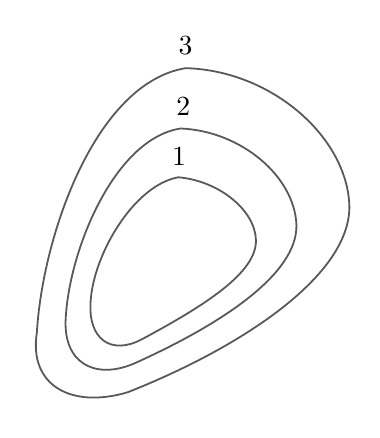
\begin{tikzpicture}[x=1.05cm,y=1.05cm]
        \tikzset{level curve/.style={draw=black!65, line width=0.65pt}}

        \draw[level curve]
            (0.15,2.40)
            .. controls (1.20,2.37) and (2.10,1.56) .. (2.13,0.74)
            .. controls (2.15,-0.10) and (0.84,-0.97) .. (-0.55,-1.52)
            .. controls (-1.22,-1.72) and (-1.75,-1.45) .. (-1.65,-0.80)
            .. controls (-1.58,0.38) and (-0.94,2.22) .. (0.15,2.40)
            -- cycle;

        \draw[level curve]
            (0.09,1.67)
            .. controls (0.82,1.64) and (1.47,1.09) .. (1.49,0.50)
            .. controls (1.50,-0.10) and (0.56,-0.71) .. (-0.49,-1.18)
            .. controls (-0.96,-1.37) and (-1.34,-1.16) .. (-1.30,-0.61)
            .. controls (-1.25,0.23) and (-0.70,1.55) .. (0.09,1.67)
            -- cycle;

        \draw[level curve]
            (0.06,1.08)
            .. controls (0.54,1.04) and (0.99,0.69) .. (1.00,0.32)
            .. controls (1.01,-0.07) and (0.40,-0.46) .. (-0.38,-0.88)
            .. controls (-0.76,-1.08) and (-1.03,-0.87) .. (-1.00,-0.43)
            .. controls (-0.97,0.14) and (-0.48,0.98) .. (0.06,1.08)
            -- cycle;

        \node at (0.07,1.33) {$1$};
        \node at (0.12,1.94) {$2$};
        \node at (0.15,2.67) {$3$};
    \end{tikzpicture}
    \caption{The first family of level curves in Exercise 3.2.}
    \label{fig:exercise-3-2-level-sets-a}
\end{figure}
